\documentclass{beamer}
\usetheme{metropolis}

\usepackage{tikz}
\usetikzlibrary{shapes.geometric, arrows}
\tikzstyle{service} = [rectangle, minimum width=2cm, minimum height=1cm, text centered, draw=black, fill=white]
\tikzstyle{flow} = [thick,->,>=stealth]
\tikzstyle{depends} = [thick,-,>=stealth]

\newcommand\TBox[3][]{%
  \tikz\node[draw,thick,text width=#2,align=left,#1] {#3};}

\title{An argumentation-based approach to summarizing discussions}
\date{}
\author{Charlie Egan}
\institute{University of Aberdeen}

\begin{document}
  \maketitle
  \begin{frame}{Itinerary}
    \begin{enumerate}
      \item{Introduction}
      \item[]{\tiny we are here \normalsize}
        \vskip 0.5em
      \item{Summary Comparison \& Feedback}
      \item{Motivations}
      \item{Extracting Points}
      \item{Generating Summaries}
      \item{Results}
      \item{Further Work}
      \item{Discussion}
	\end{enumerate}
  \end{frame}

  \begin{frame}{Summary Comparison \& Feedback}
    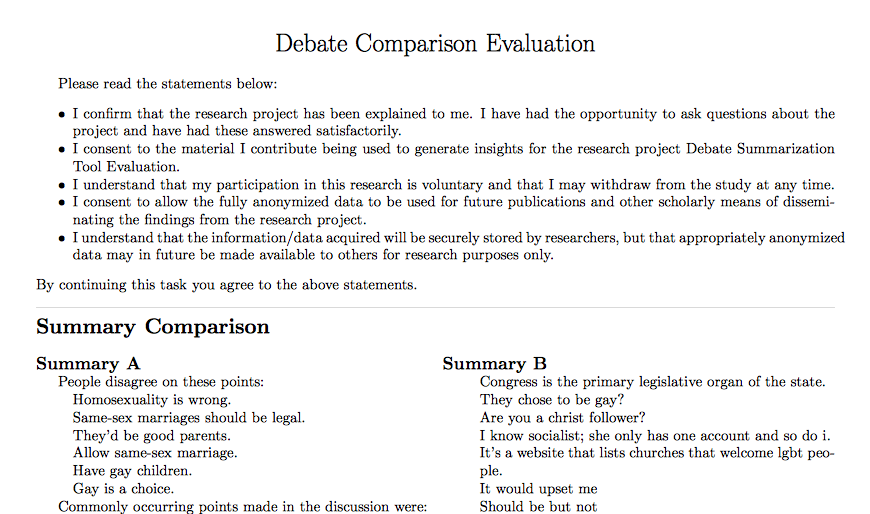
\includegraphics[width=\textwidth]{form}
  \end{frame}

  \begin{frame}{Motivations}
	\begin{center}
	  \fbox{
\includegraphics[width=\textwidth]{reddit}}

	  \fbox{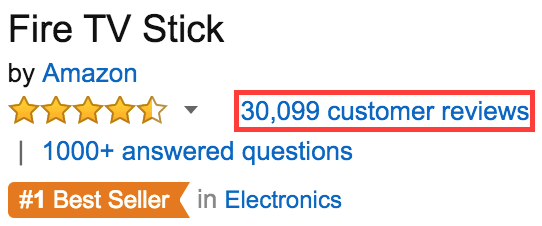
\includegraphics[width=0.5\textwidth]{fire}}

	  \fbox{
\includegraphics[width=0.6\textwidth]{indyref}}
	\end{center}
  \end{frame}

  \begin{frame}{Extracting Points (1/3)}
  	Discussion Model
	\vfill
	\TBox[fill=black!5]{10cm}{
	  Discussion \\[1ex]
	  \TBox[fill=black!10]{9.7cm}{
	  	Post \\[1ex]
		\TBox[fill=black!15]{9.4cm}{
		  Sentence \\[1ex]
		  \TBox[fill=green!5]{9.1cm}{
			Point \\[1ex]
			\TBox[fill=green!15]{2cm}{Extract}
			\TBox[fill=green!15]{2cm}{Verb}
			\TBox[fill=green!15]{3.95cm}{
			  Pattern \\[1ex]
			  \TBox[fill=green!25]{3.65cm}{Component}
			}
		  }
		}
	  }
	}
	\begin{itemize}
	  \item[]{\textbf{Extract:} ``\textit{A woman has rights.}''}
	  \item[]{\textbf{Verb:} have}
	  \item[]{\textbf{Pattern:} \texttt{woman.nsubj have.verb rights.dobj}}
	  \item[]{\textbf{Component:} \texttt{woman.nsubj}}
	\end{itemize}
  \end{frame}

  \begin{frame}{Extracting Points (2/3)}
	\begin{itemize}
	  \item[]{\textcolor{gray}{\textbf{Extract:} ``\textit{A woman has rights.}''}}
	  \item[]{\textcolor{gray}{\textbf{Verb:} have}}
	  \item[]{\textbf{Pattern:} \texttt{woman.nsubj have.verb rights.dobj}}
	  \item[]{\textcolor{gray}{\textbf{Component:} \texttt{woman.nsubj}}}
	\end{itemize}
	\begin{center}
	  Stanford Dependency Parse
	  \fbox{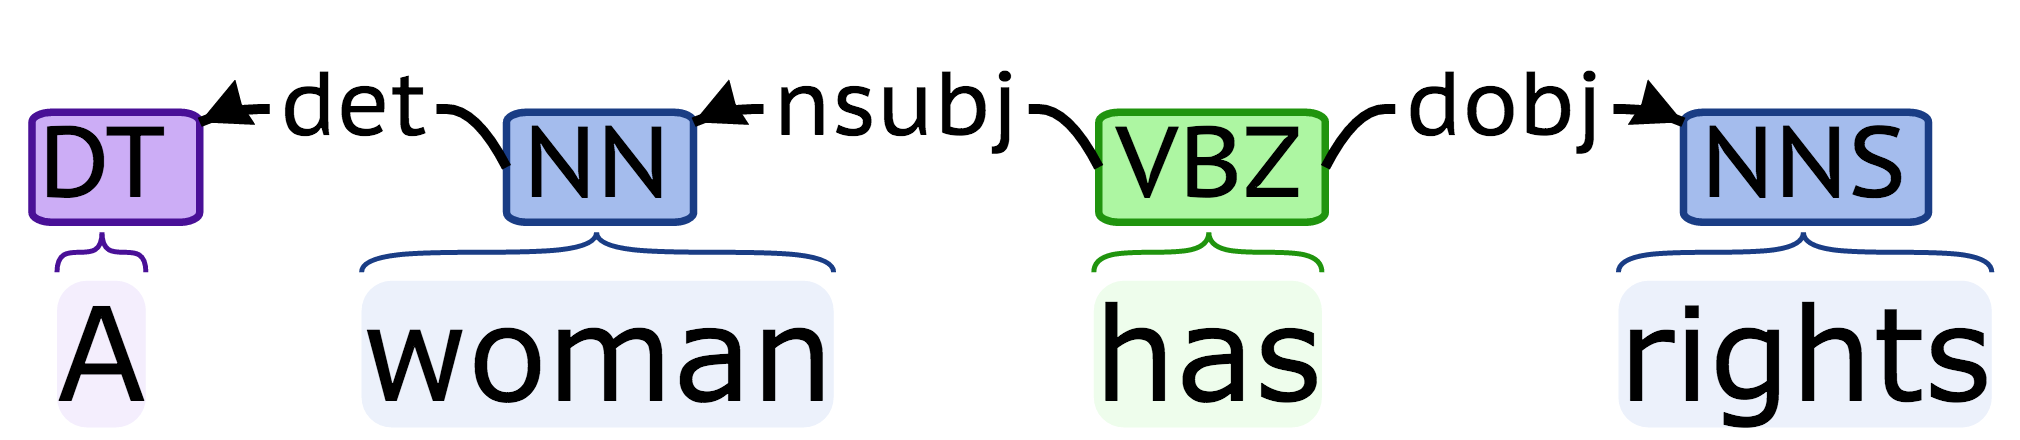
\includegraphics[width=0.7\textwidth]{depparse}}
	  \vfill
	  Lemmas

	  \fbox{
\includegraphics[width=0.6\textwidth]{lemmas}}
	\end{center}
  \end{frame}

  \begin{frame}{Extracting Points (3/3)}
	\resizebox{\textwidth}{!}{
	  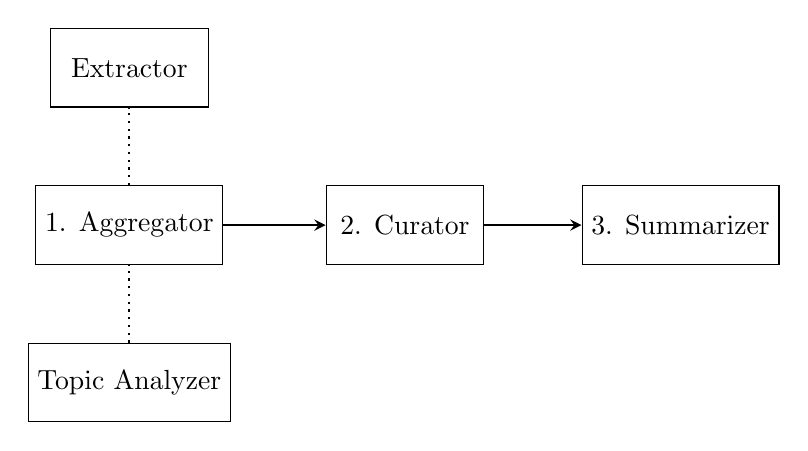
\begin{tikzpicture}[node distance=3.5cm]
		\node (agg) [service] {1. Aggregator};
		\node (top) [service, below of=agg, yshift=1.5cm] {Topic Analyzer};
		\node (ext) [service, above of=agg, yshift=-1.5cm] {Extractor};
		\node (cur) [service, right of=agg] {2. Curator};
		\node (sum) [service, right of=cur] {3. Summarizer};

		\draw [flow] (agg) -- (cur);
		\draw [flow] (cur) -- (sum);
		\draw[dotted] [depends] (agg) -- (ext);
		\draw[dotted] [depends] (top) -- (agg);
	  \end{tikzpicture}
	}
  \end{frame}

  \begin{frame}{What Next?}
    \texttt{life.nsubj begin.verb\\
      have.verb abortion.dobj\\
      abortion.nsubj be.verb legal.dobj\\
      PERSON.nsubj have.verb abortion.dobj\\
      PERSON.nsubj have.verb right.dobj\\
      fetus.nsubj be.verb person.dobj\\
      woman.nsubj have.verb right.dobj\\
      PERSON.nsubj be.verb pro-choice.dobj\\
      fetus.nsubj be.verb human.dobj\\
      PERSON.nsubj be.verb abortion.dobj\\
      abortion.nsubj be.verb murder.dobj\\
      life.nsubj begin.verb at.prep conception.dobj\\
      PERSON.nsubj be.verb pregnant.dobj\\
      life.nsubj begin.verb conception.dobj\\
      take.verb life.dobj\\
      abortion.nsubj be.verb wrong.dobj\\
      have.verb child.dobj\\
      fetus.nsubj be.verb being.dobj\\
      make.verb choice.dobj}
  \end{frame}

  \begin{frame}{What Next?}
    \fbox{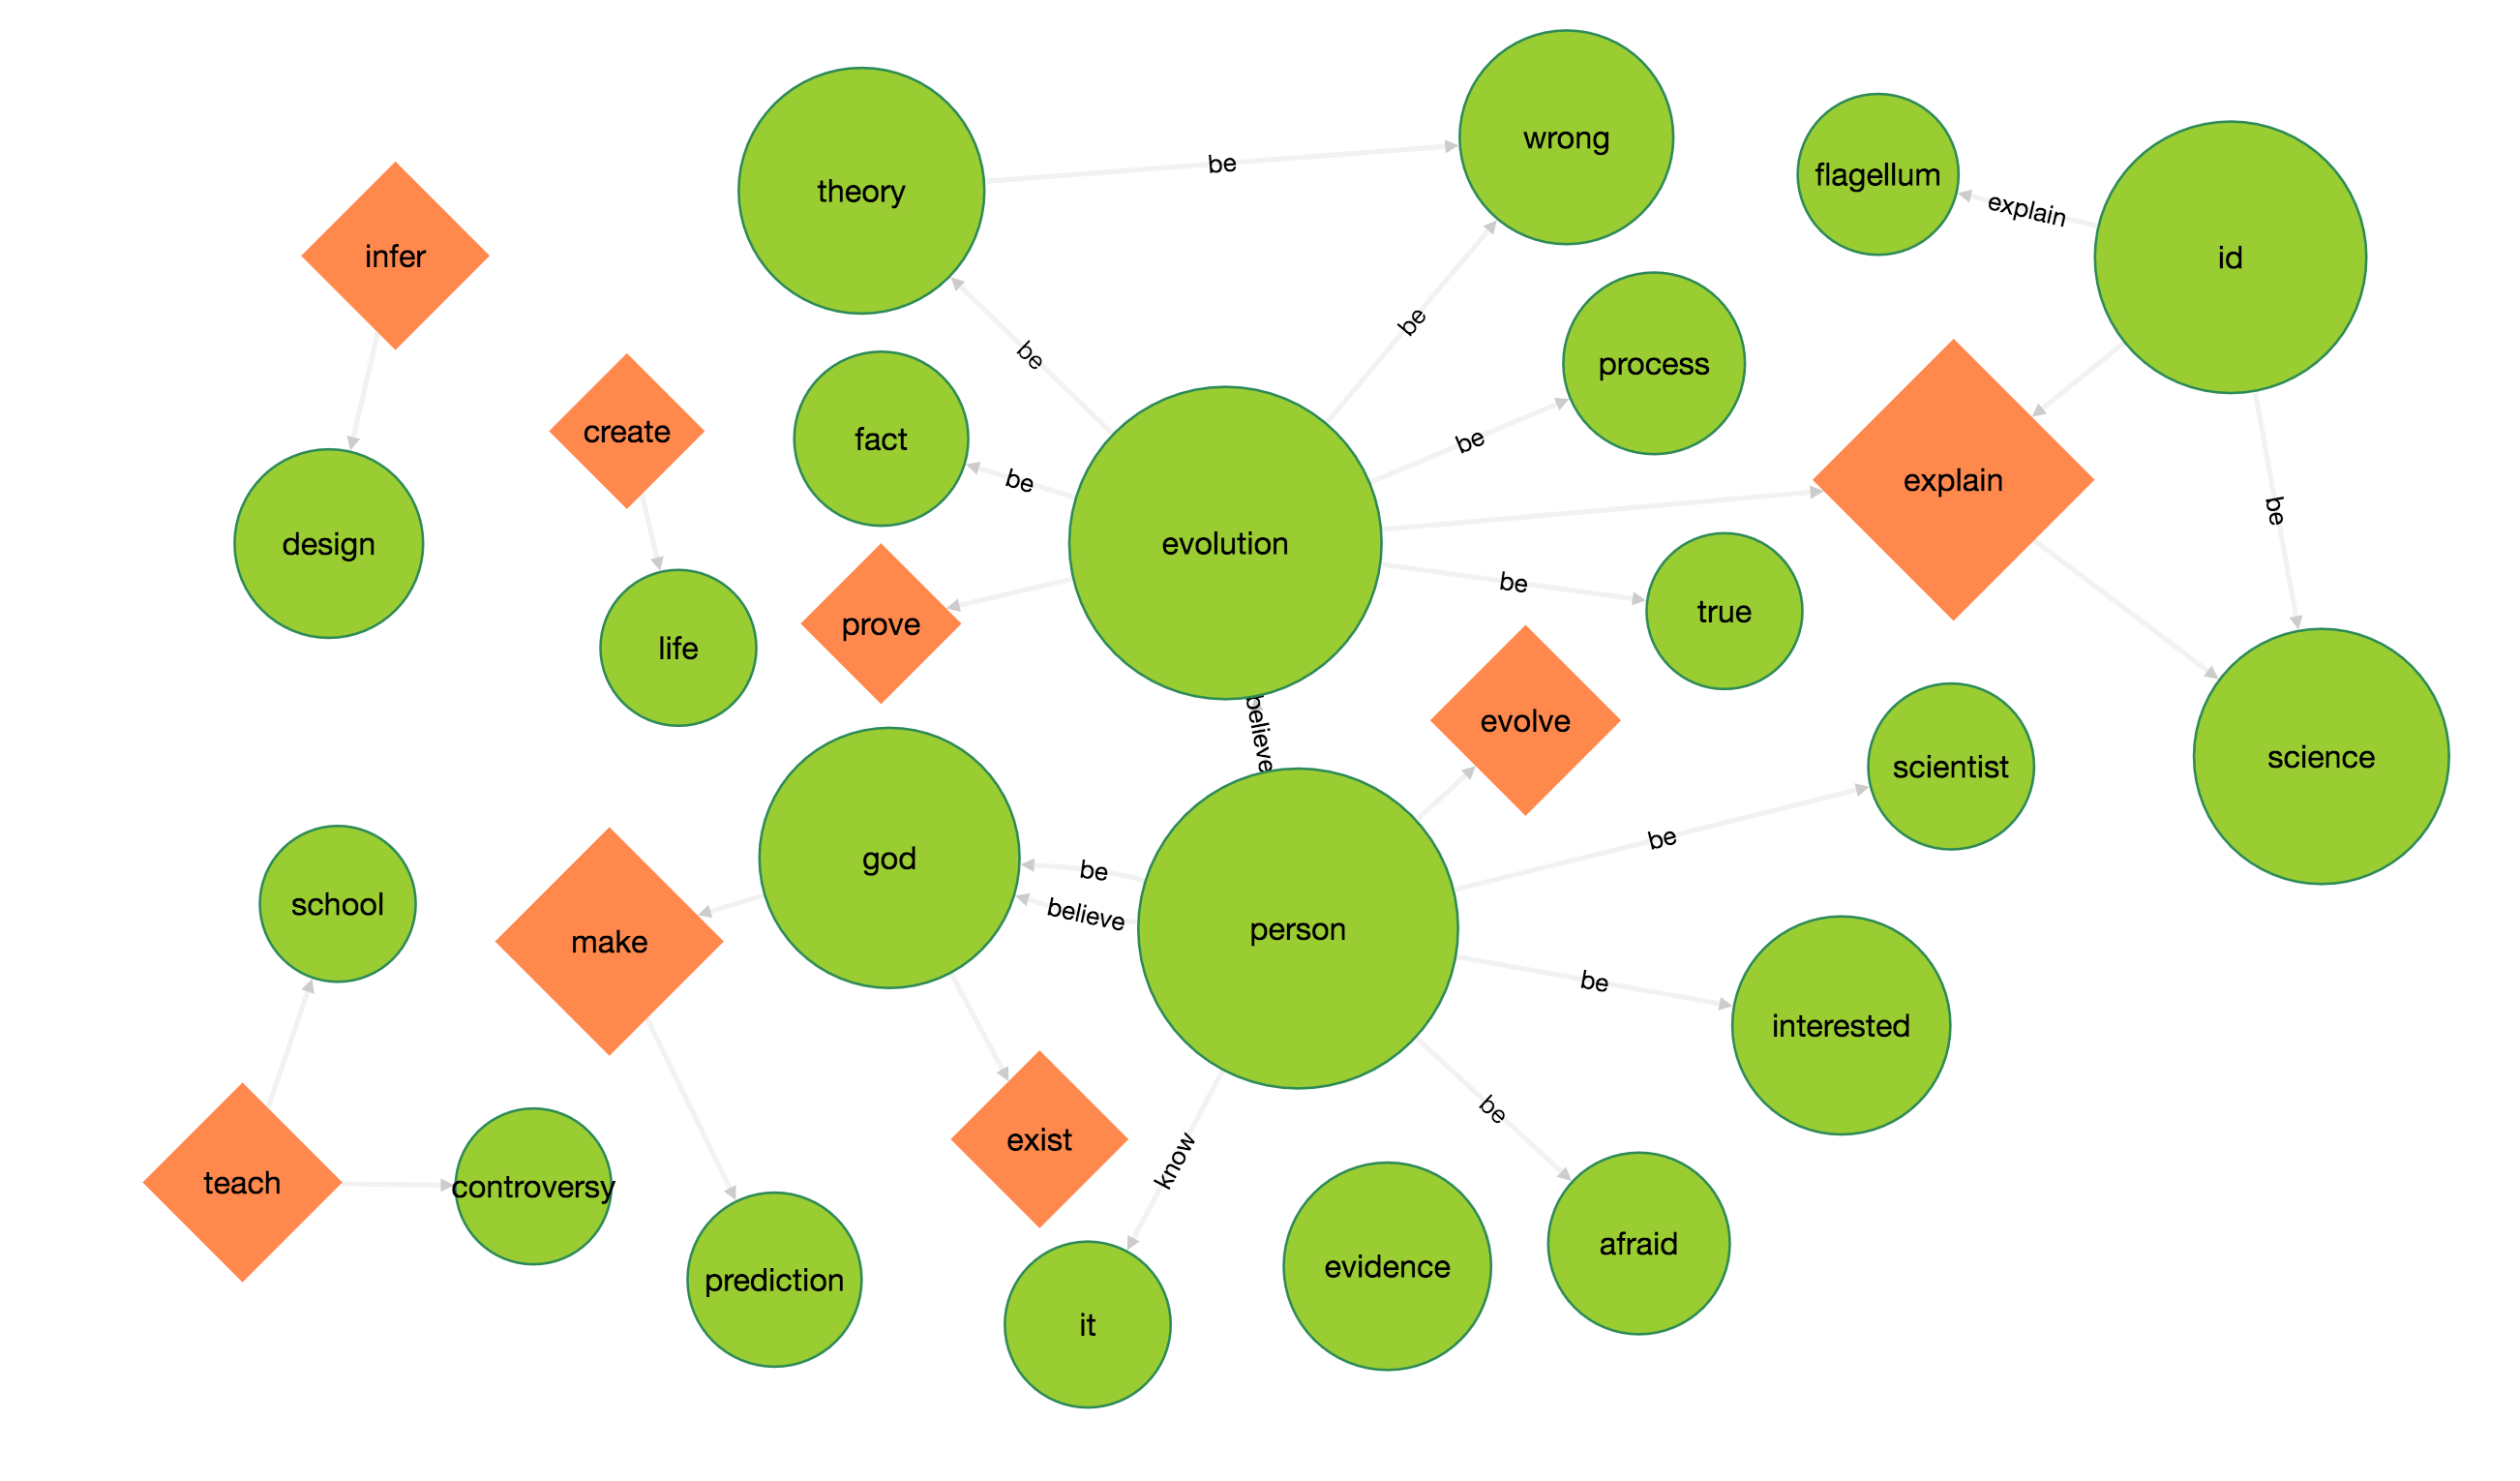
\includegraphics[width=\textwidth]{disc_graph}}
  \end{frame}

  \begin{frame}{Generating Summaries (1/4)}
    \textbf{Identifying Counter Points}

    \texttt{mother.nsubj have.verb right.dobj}\\
    \begin{center}
      using antonyms\\$\downarrow$
    \end{center}
    \texttt{\textcolor{red}{father.nsubj} have.verb right.dobj}\\
    \texttt{mother.nsubj \textcolor{red}{lack.verb} right.dobj}\\
    \texttt{mother.nsubj have.verb \textcolor{red}{left.dobj}}
  \end{frame}

  \begin{frame}{Generating Summaries (2/4)}
    \textbf{Matched Negated Points}

    \begin{center}
      ``\textit{A fetus is a human being}''
      \&
      ``\textit{A fetus is \textbf{not} a human being}''\\
      using string diffing \\$\downarrow$ \\
      ``\textit{A fetus is \textbf{\{}not\textbf{\}} a human being}''
    \end{center}
  \end{frame}

  \begin{frame}{Generating Summaries (3/4)}
    \textbf{Related Points}
  	Discussion Model
	\vfill
	\TBox[fill=black!5]{10cm}{
	  Example Discussion \\[1ex]
	  \TBox[fill=black!10]{4.65cm}{
        Post A (User 1) \\[1ex]
		\TBox[fill=red!15]{1.17cm}{\small Point 1}
		\TBox[fill=green!15]{1.17cm}{\small Point 2}
		\TBox[fill=blue!15]{1.17cm}{\small Point 3}
	  }
	  \TBox[fill=black!10]{4.65cm}{
        Post B (User 2) \\[1ex]
		\TBox[fill=green!15]{1.17cm}{\small Point 2}
		\TBox[fill=blue!15]{1.17cm}{\small Point 3}
		\TBox[fill=yellow!15]{1.17cm}{\small Point 4}
	  }
	  \TBox[fill=black!10]{4.65cm}{
        Post C (User 3) \\[1ex]
		\TBox[fill=green!15]{1.17cm}{\small Point 2}
		\TBox[fill=yellow!15]{1.17cm}{\small Point 4}
		\TBox[fill=orange!15]{1.17cm}{\small Point 5}
	  }
	  \TBox[fill=black!10]{4.65cm}{
        Post D (User 4) \\[1ex]
		\TBox[fill=red!15]{1.17cm}{\small Point 1}
		\TBox[fill=blue!15]{1.17cm}{\small Point 3}
		\TBox[fill=green!15]{1.17cm}{\small Point 2}
	  }
	}
	\vfill
    \TBox[fill=green!15]{1.17cm}{\small Point 2}
    \TBox[fill=blue!15]{1.17cm}{\small Point 3}\\
    Points 2 \& 3 are a common pair, raised together by 3 different posts.
  \end{frame}

  \begin{frame}{Generating Summaries (4/4)}
    \textbf{Other summary sections:}\\
    \begin{itemize}
      \item{Commonly occurring points}
      \item{Points that reference multiple topics}
      \item{Points with longer patterns}
      \item{Top points for core topics}
      \item{Questions asked}
    \end{itemize}
  \end{frame}

  \begin{frame}{Evaluation \& Results}
    \textbf{Evaluation Design}\\
    \begin{itemize}
      \item{Paid participants compared summaries}
    \end{itemize}
    \textbf{Results Summary}\\
    \begin{itemize}
      \item{Our layout summaries were preferred}
      \item{Methods for the selection of extracts less clear}
    \end{itemize}
  \end{frame}

  \begin{frame}{Further Work}
    \begin{itemize}
      \item{Web application interface}
      \item{Adjustments for better performance on smaller sets of text}
      \item{Improve means of selecting extracts}
      \item{Add support for hierarchical conversations and Twitter replies}
      \item{New presentations, e.g. connected graph structure}
      \item{Greater focus on argumentation structures and semantics}
    \end{itemize}
  \end{frame}

  \begin{frame}{Questions \& Discussion}
    \begin{center}
      Thanks for listening.\\
      Email: \textbf{c@egan.co} - Twitter: \textbf{@charlieegan3} \\
      \textcolor{red}{Advaith / Adam details?}
    \end{center}
  \end{frame}
\end{document}
